\documentclass[11pt,a4paper]{article}
\usepackage[utf8]{inputenc}
\usepackage[spanish]{babel}
\usepackage{amsmath}
\usepackage{amsfonts}
\usepackage{amssymb}
\usepackage{graphicx}
\usepackage{apalike}
\usepackage[left=2cm,right=2cm,top=2cm,bottom=2cm]{geometry}
\author{Barrera Vazquez Omar}
\title{\textbf{Arreglos y parámetros de amplificadores clase A\\
Sistemas electrónicos de interfaz\\
Ing. Mecatronica}}
\begin{document}
\begin{figure}
\begin{center}

\includegraphics[scale=1]{1.jpeg} 
\end{center}
\end{figure}


\maketitle


\newpage

\section{Amplificadores clase A}

Hablando de amplificadores se refiere a transistores que por medio del colector toman una corriente en continua y le dan una ganancia a la potencia de salida, la cual se observa en un apartado mas adelante de este documento. Al tipo de arreglo que se le  da en circuito a este tipo de arreglo es como se le denomina, en este documento solo tomara en consideración los de tipo A, pero se encuentran otros tipos de arreglo como los de tipo B,D,C etc. 

\subsection{Arreglo de amplificadores clase A}

Los amplificadores de tipo A normalmente tienen conectado su base a una alimentación de fuente alterna en donde se alimenta para paso a la corriente de su colector en el cual es alimentado por una tension continua y que amplifica la potencia con la que entra.

Para tener esta alimentación cuenta con una resistencia de carga conectada a una salida de tension alterna y una polarización, esto se puede observar en el siguiente esquemático:


\begin{center}
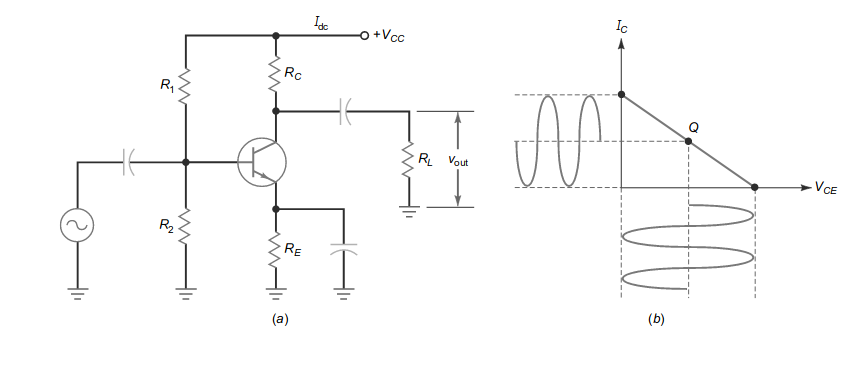
\includegraphics[scale=0.5]{1.png}
\end{center}

Se puede observar que el transistor toma la corriente del colector y le da ganancia a la salida en este caso las dos tomas a tierra, en la siguiente apartado explicaremos la ganancia de potencia que genera el amplificador.

\section{Ganancia de un amplificador tipo A}
ademas de la ganancia de tension que existe en el amplificador, esta la ganancia de la potencia en la cual se calcula de la siguiente manera; 


\begin{equation}
A_p=\frac{Pout}{Pin}
\end{equation}

La ecuación anterior nos muestra que la  \emph{ganancia de potencia} es igual a la \emph{potencia de salida} entre la \emph{potencia de entrada} en continua. Un ejemplo claro es el siguiente:

Una entrada de 10$\mu$W en la cual pasara por el amplificador, dejándole una ganancia que lo dejara con una salida de 10mW, esto lo podemos calcular de la siguiente manera;

\begin{equation}
A_p=\frac{10mW}{10"\mu"W}=1000
\end{equation}

\newpage

\section{Disipación de potencia en el transistor}

A pesar de ser una parte importante que no se puede omitir al momento de montar un amplificador, es importante considerar. Cuando un transistor no recibe ninguna señal en un base, bloquea el paso de la tension, por lo que la tension estacionaria y la corriente estacionaria es igual a la potencia de estacionaria del  transistor, en dado caso que no se tome en cuenta, si la potencia estacionaria es mayor a la de disipación lo que ocurrirá es que se estropeara el transistor. Para eso podemos calcular la disipación de potencia, con la siguiente formula:

\begin{equation}
P_Q={V_Q}{I_Q}
\end{equation}

La potencia máxima de salida es generada cuando la tension máxima de salida se genera, esto normalmente se mide con un osciloscopio el voltaje pico pico.

\section{consumo de corriente}

La fuente de alimentación continua tiene que suministrar una tension continua al amplificador, es por eso que cuenta con dos factores, el divisor de tension y la polarización, para esto es requerido saber si el amplificador es multi-etapa en caso de serlo se tiene que sumar la corrientes para encontrar el consumo de corriente total.

\section{Rendimiento del amplificador tipo A}

Para poder comparar el rendimiento de cualquier amplificador de potencia se puede utilizar la formula:

\begin{equation}
\eta=\frac{Pout}{Pdc}\times100
\end{equation}

La ecuación dicta que el rendimiento del amplificador es igual a la \emph{potencia de salida en alterna} entre las \emph{potencia de entrada en continua}  por \emph{cien}. De esta manera podemos comparar en cuestión de 0 a 100 en porcentaje dos amplificadores y ver cual tiene mejor rendimiento.

Normalmente los amplificadores de potencia no suelen tener un rendimiento mayor a 25, por lo cual para requerimientos de alta potencia en la salida, este tipo de amplificador no es de gran utilidad, pero utilización donde la salida es de baja potencia se pude utilizar de manera indiscriminada.

en sencillas palabras el rendimiento es la capacidad del amplificador de convertir su potencia en continua a potencia en alterna útil \cite{malvino}.

\begin{center}
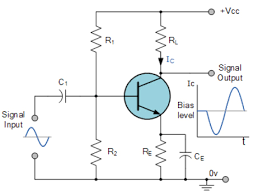
\includegraphics[scale=1]{2.png}
\end{center}







\bibliographystyle{apalike}
\bibliography{ref}  





\end{document}